\chapter{\textbf{Entorno empresarial}}

\thispagestyle{empty}

En este capítulo se describe en ambiente de la empresa Turpial Development, en
la cual se llevó a cabo la pasantía. Se presenta la misión, visión y estructura
de la empresa, así como el cargo desempeñado por el pasante durante este
período.


\section{Descripción}

Turpial Development es una empresa mediana, con cuatro años en el mercado que
está enfocada en el desarrollo de sistemas y aplicaciones web y móviles.
Fundada e integrada por jóvenes venezolanos,  ofrece soluciones que cumplen con
altos estándares de usabilidad, diseño y funcionalidad \cite{manualTurpial}.

\section{Misión}

La empresa tiene como misión “prestar servicios y consultoría en diseño y
desarrollo de soluciones web, a la medida del cliente, caracterizadas por una
alta calidad, excelente soporte y experiencia de usuario” \cite{manualTurpial} .


\section{Visión}

Su visión es “servir de plataforma para el desarrollo y éxito de nuevos
emprendimientos en el área web” \cite{manualTurpial}.

\section{Estructura}

En la figura 1.1 se muestra la estructura organizacional de Turpial
Development, la cual está conformada por cuatro departamentos:

\subsection*{Dirección de Operaciones}

Ente encargado del “funcionamiento de todos los procesos de soporte de la empresa, como administración, recursos humanos, contabilidad y compras con el fin de garantizar el correcto desarrollo de los procesos principales de la empresa" \cite{manualTurpial}.

\subsection*{Dirección de Proyectos}

Ente encargado de “atender a las necesidades y requerimientos de los clientes, sirviendo de enlace con las direcciones de desarrollo y diseño para garantizar la calidad del producto o entrega" \cite{manualTurpial}.

\subsection*{Dirección de Desarrollo}

Ente encargado de “la conceptualización y desarrollo de las necesidades del cliente, implementando e integrando el diseño acordado y las funcionalidades requeridas por dicho cliente. Se divide en tres departamentos: Conceptualización, \textit{Backend} y \textit{Frontend}" \cite{manualTurpial}.

\subsection*{Dirección de Diseño}

Ente encargado de “la conceptualización y diseño de la interfaz gráfica de los proyectos en función de las necesidades del cliente y de la mano con las decisiones tomadas por la Dirección de Desarrollo" \cite{manualTurpial}.

\begin{figure}[h]
\centering
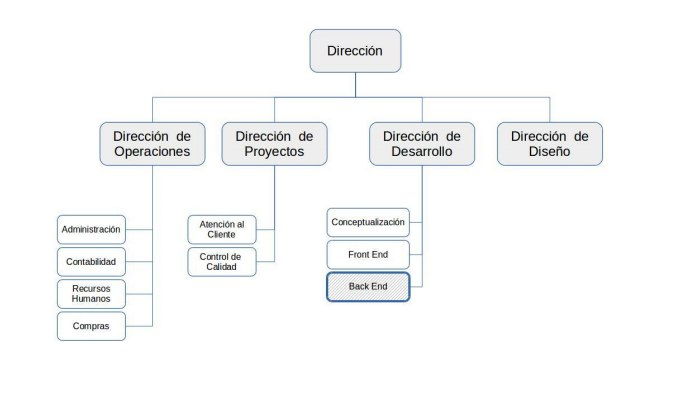
\includegraphics[width=0.9\textwidth]{Estructura_Turpial.png}
\caption{Diagrama de la estructura de Turpial Development}
\label{fig:figura1.1}
\end{figure}

\subsection*{Ubicación del pasante}

El desarrollo de la pasantía fue llevado a cabo en la Dirección de Desarrollo de la empresa. El pasante fue asignado al departamento de \textit{Backend} con el cargo de Pasante, bajo la supervisión del Tutor Industrial, el Ingeniero Pedro Romero. El pasante debe cumplir tareas tales como: levantar requerimientos, diseñar y desarrollar las funcionalidades de la solución propuesta para el sistema.
